\chapter{Introducci\'on}
La teoría de gráficas es un campo de las matemáticas ampliamente estudiado debido a la fascinante capacidad que tienen las gráficas para resolver problemas del mundo real. Las gráficas son objetos matemáticos utilizados frecuentemente como herramienta para representar y modelar diversas situaciones. Se dice que la teoría de las gráficas se originó en el siglo XVIII, específicamente al modelar el famoso problema de los puentes de Königsberg.
Para contextualizar, la ciudad de Königsberg (hoy Kaliningrado) estaba atravesada por el río Pregel, el cual formaba una isla. Además, el río se bifurcaba, generando así cuatro regiones distintas, como se muestra en la imagen. Estas regiones de tierra estaban unidas por siete puentes, y el problema consistía en trazar una trayectoria que pasara una sola vez por cada uno de los siete puentes, empezando y terminando en la misma región de tierra.
En 1735, el destacado matemático suizo Leonhard Euler resolvió este problema al modelarlo mediante una representación gráfica. Euler asignó un punto a cada región de tierra y utilizó líneas para representar los siete puentes, creando así una gráfica. Al estudiar la estructura de esta gráfica, Euler observó que había por los cuatro puntos había un número impar de puentes. Utilizando un razonamiento que ahora se conoce como el teorema de Euler, demostró que no era posible trazar una trayectoria que cruzara cada puente una sola vez y que terminara en el punto inicial.

Esta solución de Euler al problema de los puentes de Königsberg sentó las bases de la teoría de gráficas. Su enfoque para resolver el problema mediante una representación gráfica y su demostración del teorema de Euler allanaron el camino para el desarrollo de conceptos y resultados fundamentales en la teoría de gráficas. Desde entonces, la teoría de gráficas ha encontrado aplicaciones en una amplia gama de disciplinas, incluyendo la ciencia de la computación, la logística, la biología, la física y la sociología. Por ejemplo, en el ámbito de la logística, las gráficas se utilizan para determinar la ruta más eficiente para el transporte de mercancías o para la planificación de redes de distribución. Además, en la sociología, las gráficas son una herramienta valiosa para analizar y comprender las interacciones sociales, identificar líderes de opinión y comprender los patrones de difusión de información. En el campo de la informática, la teoría de gráficas es fundamental en el diseño y análisis de algoritmos. Los algoritmos de búsqueda, recorrido y optimización en gráficas son ampliamente utilizados en la resolución de problemas computacionales, como la planificación de rutas, el enrutamiento de redes y el análisis de datos en redes complejas.

En resumen, modelar un problema del mundo real mediante una gráfica nos proporciona una nueva perspectiva sobre el mismo. Podemos analizar la estructura generada por la gráfica y descubrir información y patrones que no eran evidentes inicialmente. Al reinterpretar esta información en el contexto del problema real, podemos tomar decisiones informadas sobre cómo seguir atacando nuestro problema.
Además, al interpretar los resultados de vuelta al mundo real, es posible realizar ajustes, mejoras o modificaciones en función de la comprensión obtenida a través de la modelización de la gráfica. Estos cambios pueden llevar a soluciones más eficientes, eficaces o innovadoras, y ayudar a resolver problemas de manera más efectiva.


\section{Conceptos básicos}
\label{sec:Cncpts bscs}

En esta sección, nos enfocaremos en presentar las definiciones necesarias para abordar el tema central de la tesis. Si bien esta sección puede resultar densa debido a la cantidad de definiciones, nos esforzaremos por brindar numerosos ejemplos de gráficas que faciliten la comprensión de estos nuevos conceptos.

En primer lugar, es crucial establecer un sólido fundamento conceptual para adentrarnos en el estudio de las gráficas. Por lo tanto, se presentarán las definiciones clave, empezando por la definición de gráfica así como las definiciones de vértices, aristas, tamaño y orden de una gráfica, y otros elementos esenciales para su comprensión.

Comencemos con el concepto mas fundamental, el de \indice{gráfica}.
Una \textbf{gr\'afica} \indiceSub{gráfica}{no dirigida} $G$, es un par ordenado $(V(G), E(G))$ el cual consiste de un par de conjuntos, $V(G)$ un conjunto finito cuyos elementos llamamos \indice{vértices} y $E(G)$ un conjunto cuyos elementos llamamos \indice{aristas}, los cuales son parejas no ordenadas de vértices, así $E(G)\subseteq \{ \{x,y\} \colon\ x,y\in V(G) \}$.  Si $G$ es una gráfica y $(V(G),E(G))$ son sus conjuntos de vértices y aristas, respectivamente, entonces diremos que, el \indice{orden} de $G$ es $|V(G)|$ y que $|E(G)|$ es el \indice{tamaño} de $G$.

También tenemos la definición de \textbf{gr\'afica} \indiceSub{gráfica}{dirigida}, donde el único cambio es que el conjunto de aristas son ahora pares ordenados, es decir la definición es la siguiente. Una gráfica dirigida $G=(V(G),F(G))$ es una pareja ordenada que consta de un conjunto arbitrario de vértices $V(G)$ y de un conjunto de \indice{flechas} $F(G)\subseteq \{ (x,y) | x,y\in V(G) \}$.   An\'alogamente al caso de las gr\'aficas, es posible definir orden y tama\~no para una gr\'afica dirigida.
Se suele nombrar a las gráficas dirigdas por digráficas y esta será la forma como nos referiremos a las gráficas dirigidas por el resto de la tesis. Por el momento, dejaremos de lado esta definición  y la retomaremos en capítulos posteriores.


Veamos a continuación los siguientes ejemplos.
Comencemos con $V(G)=\{1,2,3\}$  $E(G)=\{ \{1,2\} \}$. Claramente, $G. = (V(G), E(G))$ es un ejemplo de una gráfica de orden tres y de tamaño uno.   Notemos que, para expresar una gr\'afica un poco m\'as grande, por ejemplo, de orden seis y tama\~no doce, escribir a los conjuntos de v\'ertices y aristas se vuelve una labor tediosa. Por lo anterior, es deseable contar con alguna forma m\'as eficiente de representar a $G$

    
La teoría de gráficas tiene una gran ventaja respecto a otras ramas de las matemáticas, en principio, según nuestra definición de gráfica, todo es discreto, y como segunda cosa, la mayoría de nuestros objetos pueden ser representados de forma gráfica.
Por ello, haremos los siguiente.  A cada elemento de $V(G)$ lo representamos por medio de un pequeño circulo, adem\'as, cada uno tendrá una pequeña etiqueta que nos indicará de alguna forma conveniente de qué elemento de $V(G)$ se trata. Las aristas son representadas por medio de lineas, que empiezan y terminan en los círculos correspondientes a su par de vértices. Las aristas, a diferencia de los vértices, no suelen ir etiquetadas, sin embargo uno podría etiquetar a una arista con $uv$ o $vu$ si esta arista une precisamente a los vértices $u$ y $v$. Esta será la forma como se hará referencia a las aristas a lo largo de este texto.
Notemos que toda arista forzosamente se corresponde con dos vértices (no necesariamente distintos), así toda arista, debe ser dibujada con sus extremos, inicial y final, anclados en los vértices (los círculos).

\begin{figure}[H]
  \centering
  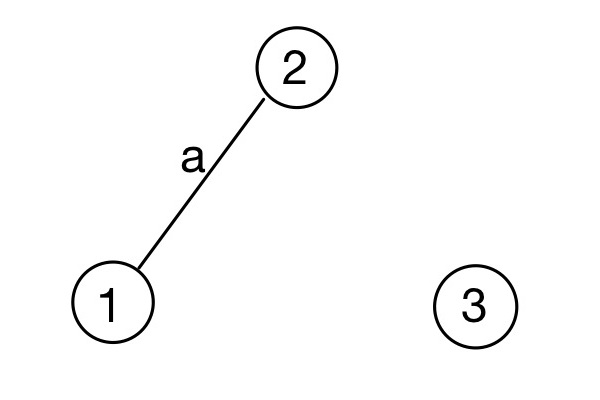
\includegraphics[width=0.4\textwidth]{recursos/capturas/01(1).jpg}
  \caption{Representación de una gráfica, de tamaño uno y orden dos.}
  \label{fig:01}
\end{figure}

Como se vio en el ejemplo anterior, puede haber algún vértice que no esté ``conectado'' a otro vértice, como el vértice 3.
Decimos que dos vértices que est\'an conectados (que pertenecen a la misma arista), como el 1 y 2, son \indiceSub{vértice}{adyacente}\textbf{s}. 
En otro caso diremos que son \indiceSub{vértice}{independiente}\textbf{s} o no adyacentes. Por ejemplo los v\'ertices 1 y 3 son independientes, y tambi\'en los v\'ertices 2 y 3 lo son.
En general, decimos que un conjunto $S\subseteq V(G)$ es  un \indiceSub{conjunto}{independiente} si y solo si, para cualesquiera v\' ertices $x,y$, si $x$ es distinto de $y$, entonces $xy\notin E(G)$.

Notemos que si $E(G)$ es el conjunto vacío, entonces, tendremos que la gráfica que obtenemos es aquella donde todos los vértices no son adyacentes entre sí.

Notemos que nuestra definición de gráfica nos permite que un arista tenga como extremos vértices iguales, aquellas aristas las llamaremos \indice{lazos}, y gráficamente las representaremos por medio de una linea curva que
termina y empieza en el mismo vértice tal como se muestra en la \cref{fig:02}, aquí los vértices 1 y 2 ambos tienen lazos.

\begin{figure}[H]
  \centering
  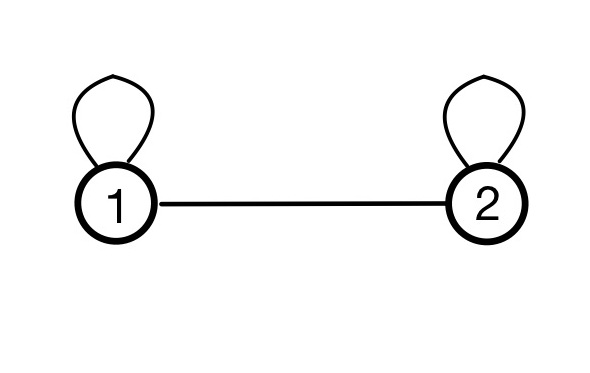
\includegraphics[width=0.25\textwidth]{recursos/capturas/02.jpg}
  \caption{Gráfica de orden dos y tamaño tres, la cual tiene dos lazos.}
  \label{fig:02}
\end{figure}

Una gráfica en la cual todos los vértices tienen lazos, la llamaremos \indiceSub{gráfica}{reflexiva}. Así la gráfica de \cref{fig:02} es una gráfica reflexiva. Por el momento trabajaremos exclusivamente con gráficas no reflexivas, a menos de que se indique lo contrario.

Veamos otro ejemplo, en \cref{fig:02} vimos que había un vértice, el cual no era adyacente a ningún otro vértice. Supongamos ahora que $V(G)$ es un conjunto cualquiera con cinco elementos, y que $E(G)$ coincide con el conjunto $\{ \{x,y\} | x,y\in V(G) \}$.
Decimos que una gráfica $G$ es una \textbf{gráfica}\indiceSub{gráfica}{ completa} si y solo si, para cada par de vértices, se tiene que estos son adyacentes. Repasando nuestras definiciones, en una gráfica completa no hay ningún par de vértices independientes, mas aún ningún subconjunto de $V(G)$ es independiente.
La gráfica resultante la podemos representar como se muestra en la \cref{fig:04}.

De forma dual a que un conjunto $S$ sea independiente, tenemos la siguiente definición, decimos que un conjunto $S\subseteq V(G)$ es un \indice{clan}, si y si solo si para todo $x,y, x\neq y, xy\in E(G)$.   

En la \cref{fig:04} se tiene que todo subconjunto de $V(G)$ es un clan.

\begin{figure}[H]
  \centering
  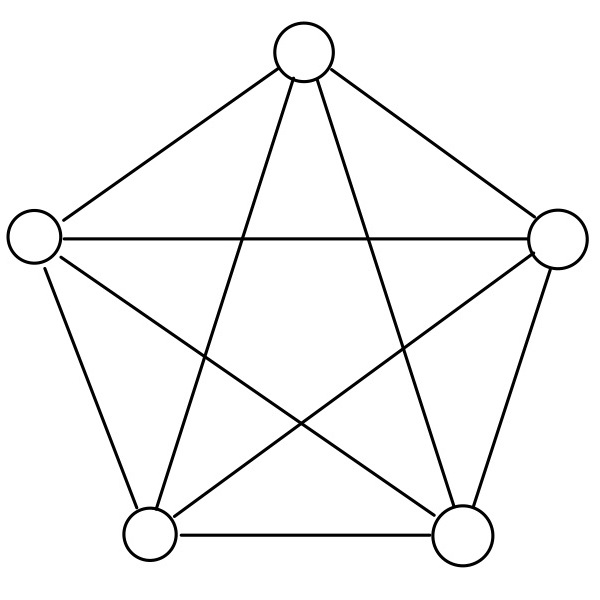
\includegraphics[width=0.25\textwidth]{recursos/capturas/04.jpg}
  \caption{Gráfica que tiene todas las aristas posibles, excepto lazos.}.
  \label{fig:03}
\end{figure}

Tenemos un par mas de definiciones.
Decimos que dos vértices $u$ y $v$ son \indiceSub{vértice}{incidente}\textbf{s} en la arista $e$, si $e$ es precisamente la arista $\{ u,v\}$.
Así en la \cref{fig:02} los vértices $u$ y $v$ son incidentes en $a$.
Otra definición mas que tenemos es la siguiente, decimos que dos aristas son \indice\textbf{arista}{adyacente}\textbf{s} si estas son de la forma $\{ u,v\}$ y $\{ v,w\}$, es decir comparten un vértice en común. Por ejemplo las aristas $a$ y $b$ son adyacentes. 

Terminaremos nuestra sección con las siguientes definiciones y ejemplos.
Dado $v\in V(G)$ definimos la \indice{vecindad} de $v$, denotada por $N(v)$ como aquel subconjunto de $V(G)$ que consta de todos los vértices adyacentes a $v$. Y al cardinal de $N(v)$ le llamamos el \indiceSub{vértice}{grado} del vértice $v$. Por otro lado definimos la \textbf{vecindad} \indiceSub{vecindad}{cerrada} de $v$ como la vecindad de $v$ unión $v$, y la denotamos con $N[v]$.
Repasemos estos conjuntos, en \cref{fig:01} la vecindad del vértice 1, $N(1)= \{ 2 \}$  así el vértice 1 tiene grado 1. Por otro lado el vértice 3, tiene grado cero ya que su vecindad es vacía.

En \cref{fig:03} notemos que todos los vértices tienen grado 4. La gráficas que cumplen que todos sus vértices tienen el mismo grado son llamadas \textbf{gráficas} \indiceSub{gráfica}{regular}\textbf{es}, si además el grado de sus vértices es $k$ las llamamos $k$-regulares. Así el ejemplo de \cref{fig:03} es una gráfica 4-regular.

\section{Subgráficas}
\label{sec:SbGrfcs}

A similitud de muchas estructuras en matemáticas, las gráficas también tienen su respectiva subestructura, así es que introducimos una subgr\'afica. 
$H$ es \indice{subgráfica} de una gráfica $G$ si sus vértices y aristas pertenecen también a $V(G)$, es decir $V(H)\subseteq V(G)$ y $E(H) \subseteq E(G) $. Decimos que un vértice $v$ es adyacente a una subgráfica $H$ si y solo si existe un vértice $u\in H$ tal que $uv\in E(G)$.

Otro concepto que surge de forma natural es el de la estructura generada por un subconjunto $S$. Por lo tanto definimos la \textbf{subgráfica} \indiceSub{subgráfica}{inducida} por $S\subseteq V(G)$, cuyo conjunto de vértices es exactamente $S$ y las aristas serán todas las aristas $\{u,v\} $ de $G$ tales que $u,v \in S$. A esta gráfica inducida la denotaremos con $V[S]$, es natural que esta es una subgráfica de $G$.

Veamos el siguiente ejemplo.
En \cref{fig:04}, tenemos una gráfica y un par de subconjuntos, el subconjunto de vértices coloreados de color verde y el conjunto de vértices coloreados de naranja. La gráfica inducida por los vértices verdes es la gráfica que se muestra en el recuadro de en medio, mientras que la inducida por el conjunto de vértices naranja es la de la derecha.

\begin{figure}[H]
  \centering
  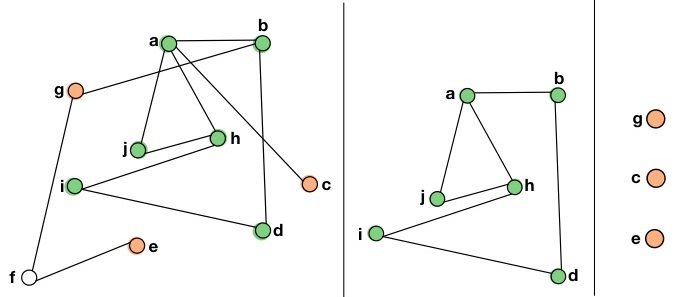
\includegraphics[width=0.7\textwidth]{recursos/capturas/09.jpg}
  \caption{Gráfica G y subgráficas inducidas $V[\{ a,b,d,i,j,h\}], V[\{ c,e,g\}]$.}.
  \label{fig:04}
\end{figure}

Denotamos por \indice{S(v)} a la gráfica generada $v$ y todos sus vecinos. Es decir $S(v)=V[N[v]]$.

Veamos el siguiente ejemplo para aterrizar el concepto.
En \cref{fig:05} al centro mostramos el conjunto $S(a)$ y a la derecha se muestra el conjunto $S(h)$.
Es importante notar que a diferencia de la vecindad cerrada de $a$, los conjuntos $S(a)$ cuentan con estructura de gráfica, mientras que las vecindades solo son conjuntos de vértices. Aquellos vértices que cumplen que $S(a)$ es una gráfica completa, son llamados \textbf{vértices} \indiceSub{vértice}{simplicial}\textbf{es}.

\begin{figure}[H]
  \centering
  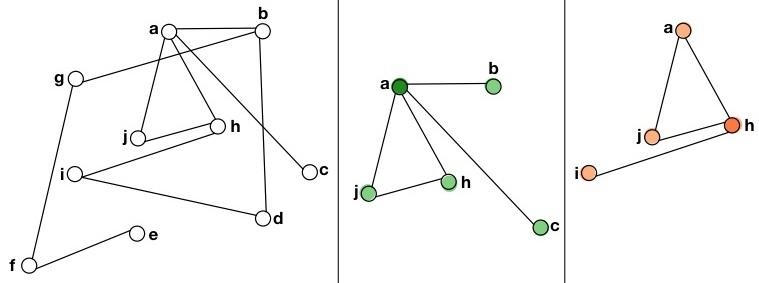
\includegraphics[width=0.73\textwidth]{recursos/capturas/10.jpg}
  \caption{Gráfica G y las vecindades cerradas $S(a)$ y $S(h)$}.
  \label{fig:05}
\end{figure}

Otros ejemplos de subgráficas son los que se obtienen al quitar vértices o aristas de una subgráfica. Sea $G$ una gráfica y $w\in V(G)$ definimos la gráfica $G-\{w\}=(V(G)-\{w\}, E')$ donde $uv\in E'$ si y solo si $uv\in E(G)$, $w\notin uv$. Dado $S\subseteq V(G)$ se puede definir inductivamente $G-S$.
Definimos también $G-\{e\}=(V(G),E')$ con $e\in E(G)$, donde $E'=E(G)-\{e\}$. Nuevamente, dado $S\subseteq E(G)$ se puede definir inductivamente $G-S$.


\section{Isomorfismos de gráficas}
\label{sec:Isomorfismos}
En esta breve sección abordamos un tema sumamente importante, estudiaremos los isomorfismos de gráficas.

Veamos el siguiente ejemplo a fin de motivar el estudio de las gráficas isomorfas.

Tomemos $V(G_1)=\{ 1,2,3\}, E(G_1)=\{ \{1,2\} \}$, $V(G_2)=\{2,3,4 \}, E(G_2)=\{ \{2,3\} \}$ y general $V(G_i)=\{ i, i+1,i+2\}, E(G_i)=\{ i,i+1\} \}$.
Esta es una familia infinita numerable de gráficas y todas ellas pueden ser representadas con la \cref{fig:01}.
Dado lo anterior nos gustaría decir que en esencia la familia anterior mencionada consta de una sola gráfica. En este punto es donde surge la definición de gráficas isomorfas, es decir si dos gráficas pueden ser representadas por el mismo dibujo, diremos que son isomorfas. 

Formalmente, decimos que dos gráficas $G$ y $H$ son \indiceSub{gráfica}{isomorfa}\textbf{s} si y solo si existe una función biyectiva $\phi \colon V(G) \to V(H)$ la cual preserva adyacencias, es decir $uv\in E(G)$ si y solo si $\phi(u)\phi(v)\in E(H)$. Una función que cumple todo lo anterior es llamado \indice{isomorfismo} de gráficas.

Así, todas las gráficas completas de orden $k$ son isomorfas entre sí.
Veamos un pequeño ejemplo de lo anterior, supongamos que $(V(G),E(G))$, $(V(H),E(H))$ son ambas gráficas completas de orden $k$, $k\in \mathbb{N}$, y para exhibir un isomorfismo entre estas gráficas solo basta exhibir una biyección entre $V(G)$ y $V(H)$, el cual sabemos que siempre existe pues los conjuntos son equipotentes.
Supongamos que $\phi: V(G) \longrightarrow V(H)$ es una biyección, quisieramos ver que $uv\in E(G)$ si y solo si $\phi(u)\phi(v)\in E(H)$, pero esto es una consecuencia inmediata del hecho de que ambas gráficas son completas.
Así concluimos que todas las gráficas completas de orden $k$, son isomorfas entre sí. Finalmente podemos decir que salvo isomorfismos existe una única gráfica completa de orden $n$, luego a la gráfica de orden $n$ la denotaremos por $K_n$.

Veamos un último ejemplo para concluir la presente sección.
En la \cref{fig:07} tenemos un par de representaciones de gráficas, y nosotros afirmamos que dichas gráficas son isomorfas, para esto exhibimos el morfismo $\phi$ tal que 
$\phi(a)=\overline{a}, \phi(b)=\overline{c}, \phi(c)=\overline{e}, \phi(d)=\overline{b}, \phi(e)=\overline{d} $.

\begin{figure}[H]
  \centering
  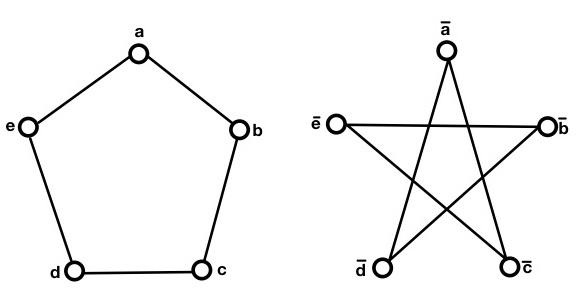
\includegraphics[width=0.6\textwidth]{recursos/capturas/11.jpg}
  \caption{Gráficas isomorfas con representaciones distintas.}.
  \label{fig:06}
\end{figure}

Así este es un ejemplo de un par de representaciones de una misma gráfica, salvo isomorfismos.

\section{Caminos y conexidad.}
\label{sec:CCyT, Conexidad}

Dada una gráfica $G$ y un par de vértices $u,v$ es bastante natural preguntarse cómo puede llegar uno del vértice $u$ al vértice $v$, siguiendo una sucesión de vértices adyacentes.
Aunque una pregunta m\'as elemental es si es posible llegar del vértice $u$ al vértice $v$ siguiendo vértices adyacentes. O m\'as a\'un, si siempre es posible llegar de cualquier v\'ertice a cualquier otro siguiendo v\'ertices adyacentes.

Dada una gráfica $G$, entendemos por un \indice{camino} a una sucesión de vértices $(u_1,u_2,...,u_n)$ donde cada par de vértices consecutivos son adyacentes, es decir $u_{i-1}u_i\in E(G)$, para cada $i \in \{2, \dots, n\}$. Un camino que empieza en el vértice $u$ y termina en el vértice $v$, lo llamamos $uv$-camino.

Un camino que no repite vértices es una \indice{trayectoria}, y un camino que no repite aristas, es un \indice{paseo}. De forma análoga una trayectoria o paseo que empieza en $u$ y termina en $v$, es una $uv$-trayectoria o un $uv$-paseo. La longitud de un camino $C$ o es el número de aristas que tiene $C$ y lo denotamos con $long(C)$, se define de la misma forma la longitud de una trayectoria y un paseo.


Por un ciclo entenderemos a un camino cuyos vértices inicial y final coinciden.

\begin{figure}[H]
  \centering
  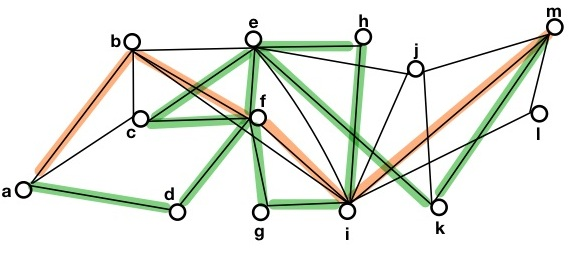
\includegraphics[width=0.6\textwidth]{recursos/capturas/12.jpg}
  \caption{En verde un $am$-camino y en naranja una $am$-trayectoria}.
  \label{fig:07}
\end{figure}

En \cref{fig:08} coloreamos de color verde el $am$-camino $(a,d,f,e,c,f,g,i,h,e,k,m)$ y tenemos de color naranja la $am$-trayectoria $(a,b,f,i,m)$.

Otro concepto importante es el de camino cerrado y ciclo. Un \indiceSub{camino}{cerrado} es un camino que cumple que su vértice inicial es igual a su vértice final. Por otro lado un camino cerrado que no repite vértices (intermedios) es un \indice{ciclo}. Se define la longitud de un camino cerrado y de un ciclo como el número de aristas que tienen estos. Al ciclo de longitud $n$, lo denotamos con $C_n$.

Adicionalmente tenemos la definición de \indice{distancia} que esta ligada a la definición de trayectoria. Así dada una gráfica $G=(V(G),E(G))$ se define la distancia entre dos vértices $u$ y $v$ como $d(u,v)=$m\'in$ \{L(C) \colon\ C$ es $uv$-trayectoria$ \}$. En caso de no existir alguna $uv$-trayectoria decimos que $d(u,v)=\infty$. 

En la parte superior de \cref{fig:09} se muestra una gráfica $G$ y un ciclo $(a,b,c,g,a)$ de longitud cuatro, y en la parte inferior de \cref{fig:09} se muestra un camino cerrado $(c,b,f,c,g,a,b,a)$ de longitud siete.

\begin{figure}[H]
  \centering
  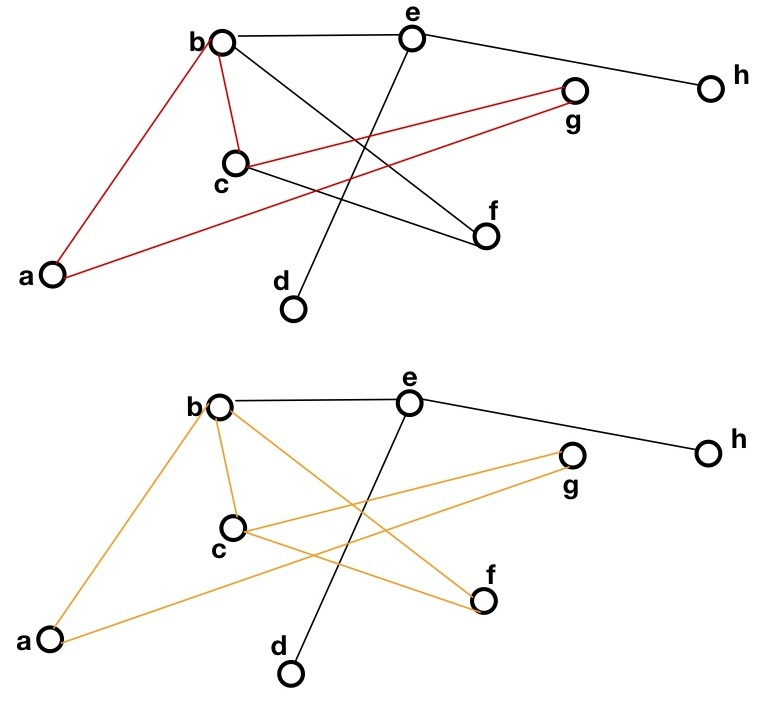
\includegraphics[width=0.6\textwidth]{recursos/capturas/13.jpg}
  \caption{Un cuatro ciclo y un siete camino cerrado.}.
  \label{fig:08}
\end{figure}

Pasemos ahora al otro concepto importante de la presente sección, el de conexidad. Decimos que dos vértices  $u$ y $v$ están \indice{conectados} si y solo si existe una $uv$-trayectoria. Si una gráfica $G$ cumple que existe una $uv$-trayectoria para todo par de vértices $u$ y $v$ de $G$, decimos que es \indiceSub{gráfica}{conexa}. Decimos que una gr\'afica es es \indiceSub{gráfica}{inconexa} si no es conexa.
Si $H$ es una subgráfica de $G$, decimos que es una \indice{componente conexa} de $G$ si no hay otra subgráfica conexa de $G$ que contenga a $H$.

Observemos \cref{fig:10}, aquí podemos ver que los vértices $d,e$ y el arista $de$ juegan un papel importante en la conexidad de la gráfica $G$, pues al remover estos vértices y esta arista, se tiene que la gráfica queda partida en dos, es decir hay vértices de $G-\{d\}, G-\{e\}$ y $G-\{ de\}$ que ya nos pueden ser conectados. Por ejemplo en ninguna de las tres gráficas anterior mencionadas existe una $af$-trayectoria, así las gráficas dejan de ser conexas.
Decimos que un vértice $v$ es un \textbf{vértice} \indiceSub{vértice}{de corte} siempre que $G-\{v\}$ es una gráfica disconexa. Y en general decimos que $S\subseteq V(G)$ es un \textbf{conjunto}\indiceSub{conjunto}{de corte} si $G-\{S\}$ es una gráfica disconexa.
Otro concepto bastante relacionado al de conjunto de corte es el de conjunto separador. Dada $G$ y $u,v\in V(G)$, decimos que $S$ es un  \textbf{conjunto} $uv$-\indiceSub{conjunto}{separador} si y solo si al considerar la gráfica $V-S$ los vértices $u$ y $v$ quedan en componentes conexas distintas. Además si no existe un subconjunto propio de $S$ que sea $uv$-separador, decimos que $S$ es un conjunto $uv$-separador mínimo. En \cref{fig:10} el conjunto $\{a,c,d\}$ es un $bf$-separador, sin embargo no es mínimo, pues por ejemplo el unitario $\{d \} \subseteq \{a,c,d\}$ y $\{d \}$ es también un $bf$-separador. 

Definimos también un \indice{puente} como un arista $uv$ tal que $G-\{uv\}$ es una gráfica disconexa.
Así en \cref{fig:10} los vértices $e,d$ son vértices de corte y el arista $ed$ es un puente. En la gráfica $G-\{ d\}$ nos quedan justamente dos componentes conexas, a saber, $C_1=V[\{a,b,c \}]$ y $C_2=V[\{g,e,f\}]$, notemos que en efecto son componentes conexas pues no existen mas subgráficas $H$ de $G$ que contengan propiamente a $C_1$ y $C_2$. 

\begin{figure}[H]
  \centering
  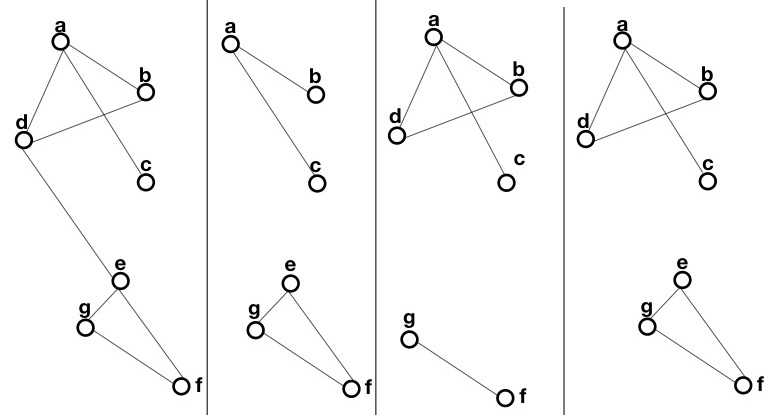
\includegraphics[width=0.8\textwidth]{recursos/capturas/14.jpg}
  \caption{Vértices de corte y puente.}.
  \label{fig:09}
\end{figure}


\section{Familias especiales de gráficas}
\label{sec:Familias especiales de gráficas}

Es usual querer agrupar a objetos matemáticos en función de sus características, así en este capítulo exhibimos familias de gráficas, las cuales comparten propiedades en común, por ejemplo podemos agrupar a gráficas en función de sus incidencias, sus propiedades de conexidad, sus grados, etc. 

\subsection{Gr\'aficas completas}

Empecemos con una familia de gráficas que ya se introdujo en \cref{sec:Cncpts bscs}, las gráficas completas de orden $n$, ya vimos que salvo isomorfismos las gráficas completas de orden $n$ son únicas y las denotamos con $K_n$, sus propiedades; cualesquiera dos vértices son adyacentes, es conexa, es cíclica, y cordal.

\subsection{Gr\'aficas multipartitas}
Sea $G=(V(G), E(G))$ una gráfica. Decimos que $(X,Y)$ es una bipartición de $G$ si y solo si $X,Y \subseteq V(G)$ y $\{X,Y\}$ es una partición de $V(G)$ tal que para toda arista $ab \in E(G)$, se cumple que $a$ est\'a en $X$ y $b$ en $Y$. Aquellas gráficas que admiten una bipartici\'on llaman gráficas bipartitas.


Veamos la siguiente gráfica de la \cref{fig:05}. Aquí es muy fácil decir cual par de conjuntos de vértices formaran la bipartición de $G$. Recordemos que, adem\'as de ser una partici\'on, una bipartici\'on debe satisfacer que toda arista $e \in E(G)$ esta tiene un extremo en $X$ y el otro en $Y$. Así, podemos proponer que $X$ consista solamente de los vértices de la parte superior y que $Y$ conste de los vértices que quedan en la parte inferior. Notemos que así las cosas, sea cual sea la arista que tomemos, esta tiene un extremo arriba y el otro queda abajo. Por lo tanto es una gráfica bipartita.

\begin{figure}[H]
  \centering
  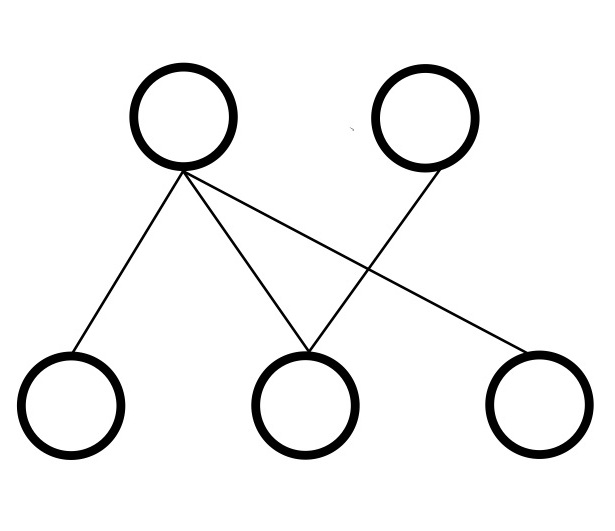
\includegraphics[width=0.25\textwidth]{recursos/capturas/05.jpg}
  \caption{Gráfica bipartita, con $X=\{$ vértices de arriba $\} $ y $Y=\{$ vértices de abajo $\}$} .
  \label{fig:10}
\end{figure}

La siguiente gráfica que expondremos es bastante interesante, pues será una gráfica bipartita la cual además cumple que todo vértice de $X$ es adyacente a todo vértice de $Y$.
Esta condición no se cumple en \cref{fig:05}, por ejemplo los dos vértices de la derecha, de arriba y abajo, no son adyacentes. Aquellas gráficas que cumplen esta propiedad, son llamadas gráficas bipartitas completas. Mas aún si $|X| = m, |Y| = n $ a le llamamos gráfica bipartita completa, y la denotamos por $K_{m,n}$.


\begin{figure}[H]
  \centering
  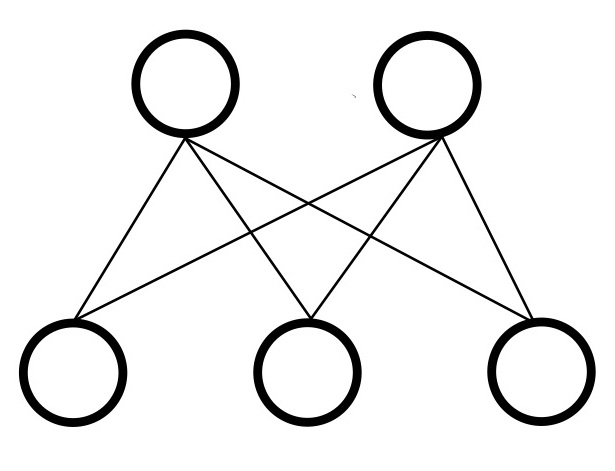
\includegraphics[width=0.25\textwidth]{recursos/capturas/06.jpg}
  \caption{Gráfica bipartita $K_{2,3}$.}
  \label{fig:11}
\end{figure}

En \cref{fig:07} tenemos otro ejemplo de gráfica bipartita.
En este ejemplo, toda bipartición será cualquier partición $(X,Y)$ de $V(G)$, en donde alguno de los dos conjuntos tiene cardinal 1. (Al ser $(X,Y)$, partición de $V(G)$, el conjunto cuya cardinalidad no sea 1, será el resto de la gráfica.)

\begin{figure}[H]
  \centering
  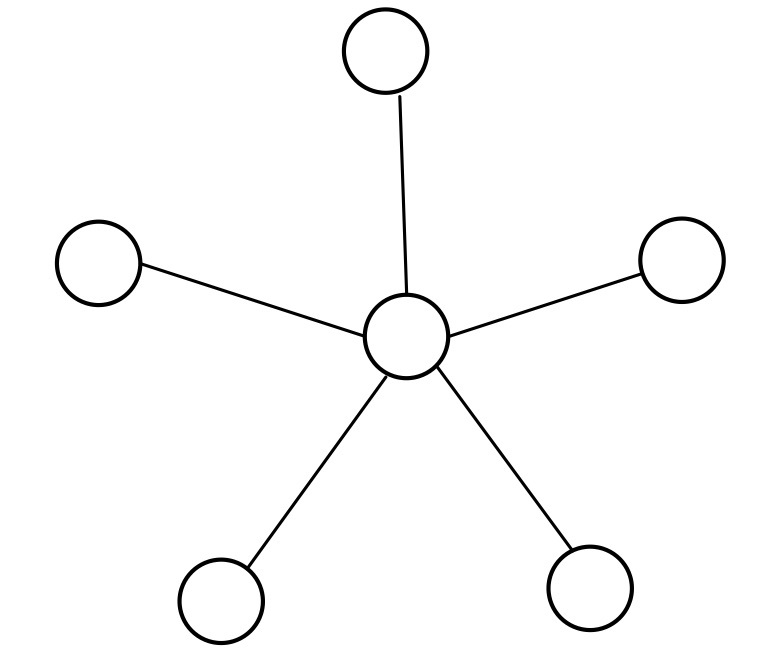
\includegraphics[width=0.25\textwidth]{recursos/capturas/07.jpg}
  \caption{Gráfica bipartita}
  \label{fig:12}
\end{figure}

Se pueden definir adicionalmente a las gráficas multipartitas, que es una generalización bastante sencilla de las gráficas bipartitas. Decimos que una gráfica $G$ es una gráfica $k$-partita si y solo si $V(G)$ puede ser particionado en $k$ conjuntos independientes, $\{W_i\}_{i=1}^n$. De forma que un arista $\{u,v\}$ es tal que $u\in W_i, v\in W_j$ con $i,j\in \{1, \dots k\}, i\neq j$ 

Veamos que \cref{fig:07} no solo es 2-partita, si no que es $k$-partita, con $2\leq k \leq 6$. La partición será de la siguiente forma. Sea $\{W_i\}$ $1\leq i\leq k-1$ una $(k-1)$-partición de $V-v_0$, donde $v_0 $ es el vértice central. Y tomamos $W_k=\{v_0\}$. Así, se tiene una $k$-partición.

Otro hecho interesante respecto a las gráficas $k$-partitas es que pueden colorearse los vértices con $k$ colores distintos de forma que no hay dos vértices del mismo color que sean adyacentes. Veamos esto en \cref{fig:15}.

\begin{figure}[H]
  \centering
  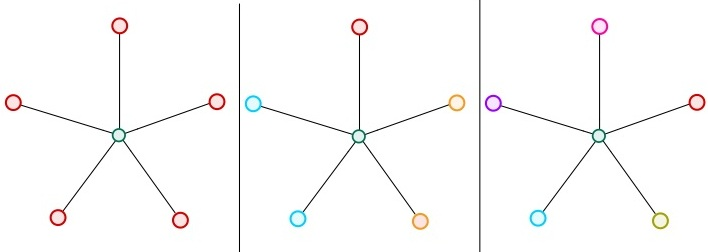
\includegraphics[width=0.8\textwidth]{recursos/capturas/15.jpg}
  \caption{Distintas coloraciones de una gráfica.}
  \label{fig:13}
\end{figure}

Las coloraciones de gráficas son ampliamente estudiadas, sin embargo las dejaremos de lado por un momento.

\subsection{\'Arboles}
Decimos que una gráfica $G$ es un árbol si $G$ es acíclica y conexa.
Esta definición depende de dos condiciones, si uno prescinde de la condición de conexidad, se obtiene la definición de bosque, es decir un bosque es una gráfica acíclica. Luego las componentes conexas de un bosque son justamente árboles.

\begin{figure}[H]
  \centering
  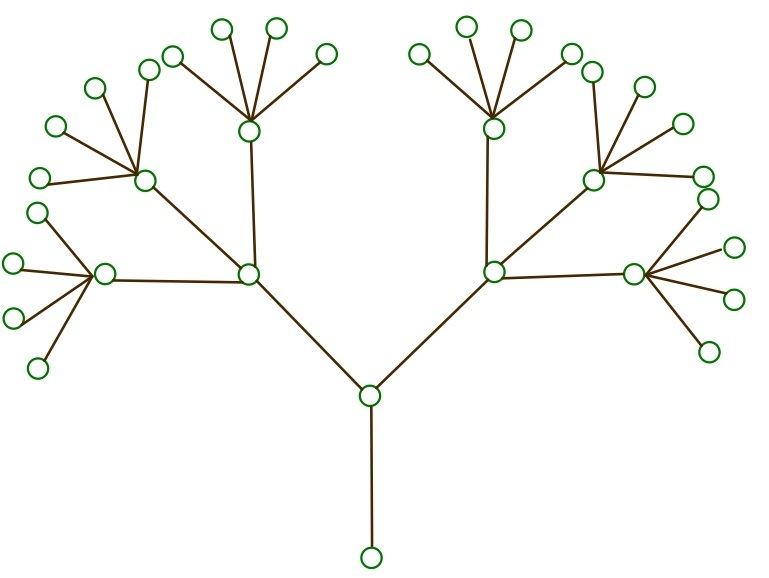
\includegraphics[width=0.5\textwidth]{recursos/capturas/16.jpg}
  \caption{Árbol.}
  \label{fig:14}
\end{figure}

Es relativamente fácil encontrar ejemplos de árboles, y mas aún teniendo varios de éstos, es más fácil aún dar ejemplos de bosques. Recordemos que los bosques solo son aquellos que sus componentes conexas son árboles.

Los árboles tienen una gran cantidad de caracterizaciones, el siguiente teorema ilustra varias de estas.

\begin{teorema}
\label{teo:101}
    Sea $G$ una gráfica las siguientes proposiciones son equivalentes;\\
    i) $G$ es un árbol.\\
    ii) $G$ es conexa y tiene $n-1$ aristas.\\
    iii) $G$ es conexa y toda arista de $G$ es un puente.\\
    iv) Dados $u,v$ un par de vértices independientes de $G$, existe exactamente un ciclo en $G\cup \{uv\}$.
\end{teorema}

Tenemos también el concepto de árbol generador. Así dada una gráfica $G$ decimos que $T$ es un árbol generador si $T$ es una subgráfica de $G$ la cual es un árbol y $T$ genera a $G$.
Una consecuencia inmediata de que una gráfica $G$ cuente con un árbol generador, se traduce a que $G$ es una gráfica conexa. También se sabe que toda gráfica conexa posee un árbol generador.

\begin{figure}[H]
  \centering
  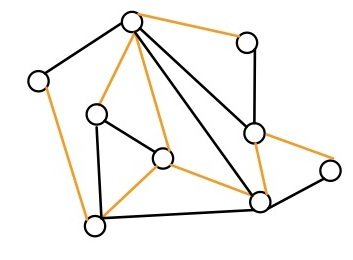
\includegraphics[width=0.4\textwidth]{recursos/capturas/17.jpg}
  \caption{Árbol generador en naranja.}
  \label{fig:15}
\end{figure}


\subsection{Gr\'aficas cordales}
Las gráficas cordales juegan un papel de gran importancia respecto a la gráficas de intervalos en \cref{cap:GrafInt} veremos que ser gráfica cordal es una necesidad para las gráficas que son de intervalos. 

Dada una gráfica $G$, decimos que es \indiceSub{gráfica}{cordal} si todo ciclo de longitud mayor o igual a cuatro tiene una cuerda, es decir, un arista de $G$ que no pertenece al ciclo pero que si une a dos vértices del ciclo. En \cref{fig:09} el único $4$-ciclo no tiene cuerdas, luego $G$ es no cordal.

Las gráficas cordales tienen varias propiedades las cuales ayudan a caracterizarlas. Una de las primeras características que tiene las gráficas cordales es la siguiente.

\begin{teorema}
\label{teo:103}
    Toda gráfica cordal $G=(V,E)$ tiene un vértice simplicial. Mas aún si $G$ no es una gráfica completa entonces esta tiene un par de vértices smpliciales no adyacentes.
\end{teorema}

\begin{proof}
    Si $G$ es una gráfica completa entonces cualquier vértices es simplicial. Por lo tanto probemos vía inducción sobre el orden de $G$ que; si $G$ tiene un par de vértices $a,b$ no adyacentes y es cordal, entonces $G$ tiene un par de vértices simpliciales no adyacentes. Supongamos entonces que para toda gráfica de orden menor que $G$ se tienen dos vértices simpliciales. Sea $S$ un $ab$-separador mínimo y denotemos con $A,B$ a las componentes conexas de $G-S$ que contienen a $a$ y $b$ respectivamente. Tenemos que $G[C \cup S]$ tiene dos vértices simpliciales para $C\in \{A,B\}$ o bien $G[C \cup S]$ es una gráfica completa, en el primer caso alguno de los dos vértices simpliciales debe pertenecer a $C$ pues $S$ es completa como consecuencia del teorema anterior. En el segundo caso, todo vértice de $S$ es simplicial en $G[C \cup S]$. Dado que $V[C]\subseteq G[C \cup S]$ se tiene que todo vértice simplicial de $G[C \cup S]$ que esté en $C$ es simplicial en $G$, así se tiene que hay dos vértices simpliciales.
\end{proof}

\begin{teorema}
    Cada gráfica finita cordal contiene un vértice simplicial.
\end{teorema}

\begin{proof}
    Prueba por inducción sobre el orden de $G$.\\
    Claramente si el orden de $G$ es uno, hay un punto simplicial, a saber el único vértice de $G$.
    
    Supongamos entonces que toda gráfica finita acíclica de orden menor a $n$, $n\in \mathbb{N}$, satisface tener un vértice simplicial.

    Veamos ahora que una gráfica $G$ finita acíclica de orden $n$ tiene un punto simpicial.
    Sea $b\in V(G)$ un vértice arbitrario, y a continuación consideremos $G_1=G-\{b\}$, por hipótesis inductiva sabemos que existe un $a\in G_1$ que es un vértice simplicial, llamemos $S_1(a)=[S(a)]_{G_1}$.
    En este punto notemos los siguientes tres casos; \\
    i) Si $a, b$ no son adyacentes, entonces tenemos que $a$ es también simplicial en $G$. Y tenemos el resultado que buscábamos.\\
    ii) Si existe algún $c\in S_1(a)$ no tiene vecinos en $G-S_1(a)$, entonces $S(c)=S_1(a)$, que sabemos que es una gráfica completa, y por consecuencia $c$ es vértice simplicial de $G$.\\
    iii) Como último caso trivial se tiene que si $b$ es adyacente a todos los puntos de $S_1(a)$ entonces $S(a)=S_1(a) \cup \{b\}$ y entonces $a$ es simplicial. \\
    Por todo lo anterior nos centraremos a considerar el caso en el que;\\
    I) $ab \in E(G)$ \\
    II) $\forall c\in S_1(a), c\neq a, (N(c)\nsubseteq S_1(a))$\\
    III) $\exists c_0 \in S_1(a), c\neq a,(c_0b\notin E(G))$\\
    Consideremos $G-S_1(a)$, esta gráfica no es conexa necesariamente, por lo cual, llamamos $C_1$ a la componente conexa de $G-\{S_1(a)\}$ que contiene a $b$. Llamamos $C_2$ a $G-\{C_1 \cup S_1(a)\}$. \\
    A continuación probaremos que si $c\in S_1(a)$ y $c$ es vecino a la componente $C_1$, entonces $cb\in E(G)$.
    Así las cosas sea $c\in S_1(a)$, tal que $c$ es vecino de la subgráfica $C_1$, y tomemos $d_1\in C_1$ un vértice adyacente a $c$. Notemos que si $c=a$ o $d_1=b$ entonces es inmediato que $cb\in E(G)$. Por lo que supondremos que $c \neq a$ y $d_1\neq b$. Como primer punto, tenemos que dado que $C_1$ es una componente conexa, y $d_1,b\in C_1$ entonces existe una trayectoria $d_1,\dots,d_k,b$ en $C_1$ con $b\neq d_i$ para todo $i\in \{1,\dots , k\}$. Por otro lado dado que $a,b$ son adyacentes, se tiene que $b,a,c,d_1,\dots,d_k,b$ es un ciclo. Además se tiene que $a\neq d_i$ y $ad_i\notin E(G)$ para todo $i\in \{1,\dots , k\}$.
\end{proof}

La primer caracterización que exhibimos, nos habla sobre dar un orden de los vértices de $G$.

Sea $G$ una gráfica y sea $\sigma= [v_1,v_2, \dots, v_n]$ una ordenación de los vértices de $G$. Decimos que $\sigma$ es un \indice{esquema perfecto de eliminación de vértices} si y solo si el vértice $v_i$ es un vértice simplicial de la gráfica inducida $V[v_{i}, \dots , v_n]$.

Un ejemplo de una gráfica con un esquema perfecto de eliminación de vértices lo mostramos en \cref{fig:16}, el esquema $\sigma=[1,2,\dots, 10]$ es un esquema perfecto de eliminación vértices. Veamos que; el vértice $1$ es un vértice simplicial en $G$, el vértice $2$ es un vértice simplicial en $G[2, \dots, 10]$, análogamente el $3$ es un vértice simplicial en $G[3, \dots, 10]$ y así consecutivamente. 

Notemos que una gráfica puede tener mas de un esquema perfecto de eliminación de vértices. En el ejemplo anterior citado $\phi = [1,3,2,4,5,6,7,8,9,10]$ es otro esquema perfecto de eliminación de vértices. En realidad siempre podemos empezar un esquema perfecto de eliminación de vértices a partir de un vértice simplicial (en la gráfica inducida por los vértices restantes).

\begin{figure}[H]
  \centering
  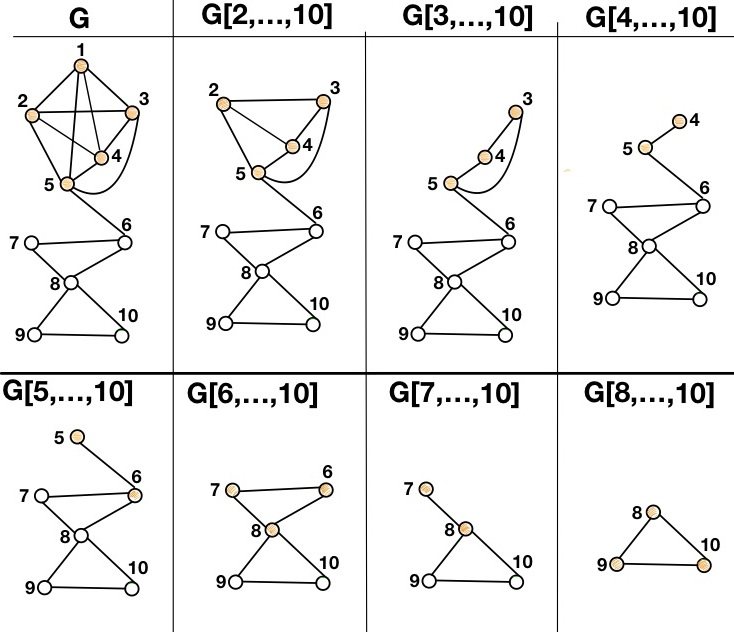
\includegraphics[width=0.75\textwidth]{recursos/capturas/19.jpg}
  \caption{Esquema perfecto de eliminación de vértices. En naranja se muestran los $S(i)$.}
  \label{fig:16}
\end{figure}

Así tenemos el siguiente teorema. 

\begin{teorema}
\label{teo:102}
    Sea $G$ una gráfica. Las siguientes proposiciones son equivalentes.\\
    i) $G$ es una gráfica cordal.\\
    ii) $G$ tiene un esquema perfecto de eliminación de vértices.\\
    iii) Cada vértice mínimo separador de vértices induce una subgráfica completa de $G$.
\end{teorema}

\begin{proof}
    iii) $\Rightarrow$ i)
    Sea $[a,x,b, y_1, \dots, y_n, a]$ un ciclo simple de $G$. Cualquier $ab$-separador debe contener a los vértices $x,y_i$ para alguna $i\in \{1, \dots, n \}$, luego al pertenecer a un $ab$-separador y al tener por hipótesis que los separadores inducen subgráficas completas, se tiene que $xy_i \in E(G)$, luego $[a,x,b, y_1, \dots, y_n, a]$ tiene una cuerda.\\
    
    i) $\Rightarrow$ iii) 
    Supongamos que $S$ es un $ab$-separador mínimo y denotemos con $A,B$ a las componentes conexas de $G-S$ que contienen a $a$ y $b$ respectivamente. Dado que $S$ es minimal debe suceder todo elemento $x\in S$ es vecino de $A$ y de $B$. Por lo tanto para cada par de vértices $x,y\in S$ existen los caminos $[x,a_1, \dots, a_r,y]$ y $[y,b_1,\dots, b_t,x]$ de tal forma que $a_i\in A, b_i\in B$ y además son elegidos de forma que las longitudes de estos es mínima. Luego al concatenar los caminos anteriores, obtenemos el ciclo $[x,a_1, \dots, a_r,y,b_1,\dots, b_t,x]$ el cual es un ciclo de longitud al menos 4, luego por hipótesis tenemos que debe haber una cuerda. De aquí notamos que $a_ib_j\notin E$ pues $A$ y $B$ están en componentes distintas. También $a_ia_j, b_ib_j \notin E$ para $i,j$ no consecutivos, dada la minimalidad de las trayectorias. Por lo tanto la unica cuerda posible es $xy$.
    
\end{proof}

Para concluir la prueba \cref{teo:202} probaremos un teorema auxiliar.
Una vez teniendo este teorema, regresamos a la prueba del \cref{teo:202}. 
\begin{proof}
    i) $\Rightarrow$ ii) 
    Probemos esto por inducción. Supongamos que toda gráfica cordal de grado menor al de $G$ tiene un esquema perfecto de eliminación de vértices. Probemos que $G$ en efecto tiene un esquema perfecto de eliminación de vértices. Usando \cref{teo:203}, tenemos que $G$ tiene un vértice simplicial $x$. Al considerar $G-\{x\}$ tenemos una gráfica cordal luego por inducción $G-\{x\}$ cuenta con un esquema perfecto de eliminación de vértices $\sigma $. Para obtener un esquema perfecto de eliminación de vértices de $G$, basta adjuntar a $\sigma$ el vértice $x$ como prefijo.
    ii) $\Rightarrow$ i) 
    
\end{proof}

Tenemos la propiedad probada por Dirac, la cual establece que toda gráfica cordal tiene al menos un vértice simplicial. En cuanto a las caracterizaciones de las gráficas cordales, tenemos que toda gráfica cordal tiene un esquema perfecto de eliminación de vértices, dicho esquema lo definimos mas adelante. Otra caracterización mas es el hecho de que todo conjunto minimo separador de vértices induce una gráfica completa y 



\begin{comment}
En la \cref{fig:17} mostramos una gráfica la cual $\sigma = [a,e,b,f,c,g,d]$ es  un esquema perfecto de eliminación de vértices. Notemos que una gráfica puede tener mas de un esquema perfecto de eliminacióin de vértices, por ejemplo en la anterior citada $\phi = [d,g,c,f,b,e,a]$ es otro esquema perfecto de eliminación de vértices.

\begin{figure}[H]
  \centering
  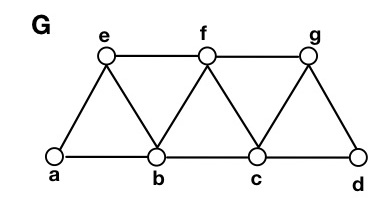
\includegraphics[width=0.5\textwidth]{recursos/capturas/18.jpg}
  \caption{Árbol generador en naranja.}
  \label{fig:17}
\end{figure}  
\end{comment}


\begin{comment}
\section{C\'omo usar esta plantilla}
\label{sec:howto}

Esta plantilla se dise\~n\'o como una ayuda para aquellos usuarios que ya
est\'an familiarizados con \LaTeX, pero nunca han desarrollado un proyecto
``grande'' (m\'as all\'a de tareas o reportes finales de proyectos).   Siguiendo
las instrucciones encontradas en el archivo \ttt{README.md}, lo m\'as probable
es que hayan creado un nuevo repositorio a partir del ``template repository''
que contiene este proyecto.   En primer lugar, verifique que el proyecto compile
adecuadamente; el proyecto deber\'ia de compilar sin errores ni advertencias. Es
posible que la primera vez que se compila, su manejador de paquetes actualice
varios de \'estos, lo que puede llevar un tiempo.   En caso de tener errores, es
posible que \'estos se deban a la falta de algunos paquetes, y a que su
manejador de paquetes no los instala autom\'aticamente;  instalar los paquetes
faltantes manualmente deber\'ia de resolver todos los problemas.

La estructura de este proyecto es sencilla.   Hay un archivo central,
\ttt{tesis.tex}, que contiene el pre\'ambulo del documento, y donde se incluyen
todos los paquetes y definiciones necesarias.   El c\'odigo est\'a comentado,
explicando de forma m\'inima para qu\'e sirve cada comando; se recomienda que al
modificarlo se mantenga un estilo semejante para no causarle problemas
innecesarios a su yo del futuro.   Todos los contenidos se encuentran en otros
archivos dentro del mismo directorio, que son llamados desde \ttt{tesis.tex}
mediante el comando \ttt{\textbackslash{include}}.   De esta forma se
incluyen la car\'atula, la hoja de datos, los cap\'itulos que forman parte de la
tesis, la bibliograf\'ia, etc.   Por otro lado, \LaTeX~ genera (casi)
autom\'aticamente el \'indice y el \'indice alfab\'etico, pero hay que agregar
comandos para su inclusi\'on.  La mayor\'ia de los usuarios s\'olo necesitan
preocuparse por modificar algunos de los archivos existentes, e incluir otros.
Sin embargo, es \'util que est\'en familiarizados con los conceptos de
\ttt{frontmatter}, \ttt{mainmatter}, \ttt{appendix} y \ttt{backmatter} (puede
referirse a \cite{oetiker2007} para revisarlos).

A continuaci\'on, se recomienda revisar el documento generado (este documento) e
identificar cu\'ales son las caracter\'isticas que se desean utilizar (dibujos,
algoritmos, tablas, etc.).   Tras determinar cu\'ales son los paquetes
relevantes para las caracter\'isticas deseadas, comentar (o borrar) todos
aquellos que no ser\'an utilizados en el archivo \ttt{tesis.tex}.   Si se est\'a
usando \ttt{git}, se recomienda leer \cref{sec:git}.   De otro modo, puede
empezar a reemplazar los contenidos de la plantilla con su propio trabajo.

\section[Uso recomendado con git]{Flujo de trabajo recomendado con \ttt{git}}
\label{sec:git}

Si el lector no est\'a usando \ttt{git}\index{git}, puede ignorar esta
secci\'on.   De otro modo, se propone un flujo de trabajo con el que el tesista
puede autogestionar el desarrollo de su tesis, o \'este puede ser supervisado
por su director de tesis mediante el uso de \ttt{GitHub}\index{git!GitHub}.

Este repositorio cuenta con dos ramas al momento de ser clonado: \ttt{master} y
\ttt{original}.   Idealmente, \ttt{master} debe contener su trabajo final, una
vez que ha sido revisado por su director de tesis, por lo que nunca deber\'ia de
trabajar directamente sobre esta rama.   Por este motivo, antes de realizar
cambios y experimentos en los archivos del proyecto, se recomienda crear una
nueva rama, llamada por ejemplo \ttt{prueba}, usando el comando \ttt{git
checkout -b prueba}.   Tras realizar algunos experimentos, eliminar los
contenidos que no necesita, y agregar sus datos a la car\'atula y hoja de datos,
posiblemente se sienta listo para empezar a incluir su trabajo en el proyecto.
En este momento se recomienda agregar los cambios realizados al repositorio,
realizar un \ttt{commit} con los mismos, y realizar un \ttt{merge} a
\ttt{master}.   A partir de ahora, \ttt{master} estar\'a lista para empezar a
trabajar.

En este momento, es posible crear
\href{https://guides.github.com/features/issues/}{\ttt{Issues}} en su
repositorio para tener metas de trabajo.   Como muy posiblemente s\'olo una
persona est\'e trabajando en el proyecto (el tesista), es posible que s\'olo
se trabaje en un \ttt{issue} a la vez, sin embargo, es una buena pr\'actica
tener una rama para cada \ttt{issue} (lo que resultar\'a a\'un m\'as \'util si
se trabaja en m\'as de una caracter\'istica nueva a la vez).   Idealmente, toda
rama nueva saldr\'a de \ttt{master}, y estar\'a dedicada a resolver un \'unico
\ttt{issue}.   Un ciclo de trabajo\index{ciclo de trabajo} usual puede verse
de la siguiente forma.

\begin{enumerate}
  \item Determinar una caracter\'istica nueva que se desea agregar al
    trabajo (e.g., la demostraci\'on de un teorema central de la tesis).

  \item Crear un \ttt{issue} describiendo qu\'e es lo que espera agregar
    al trabajo (e.g., qu\'e conceptos se necesitan agregar, proveer una
    referencia del teorema, indicar si es necesario incluir resultados
    preliminares o ejemplos).

  \item Asignar el \ttt{issue} al tesista, y opcionalmente agregar una fecha
    l\'imite.   (En caso de que el director de tesis est\'e supervisando el
    trabajo mediante \ttt{git}, asignarlo como revisor del \ttt{issue}.)

  \item Crear una nueva rama (a partir de \ttt{master}) para resolver el
    \ttt{issue}.

  \item Una vez resuelto el \ttt{issue}, hacer un \ttt{commit} (o varios) con
    los cambios, un \ttt{push} al repositorio, y abrir un \ttt{pull request}
    que ser\'a cerrado una vez que el director de tesis haya revisado el nuevo
    trabajo. (En caso de que el director de tesis est\'e supervisando el
    trabajo mediante \ttt{git}, deber\'a de ser agregado como revisor del
    \ttt{pull request}, y \'este ser\'a mezclado hasta tener su aprobaci\'on.)

  \item Tras aceptar el \ttt{pull request}, cerrar el \ttt{issue} y borrar la
    rama correspondientes (esto puede hacerse autom\'aticamente al aceptar el
    \ttt{pull request}).
\end{enumerate}

Un ciclo de trabajo tomar\'a tipicamente una semana, por lo que las metas a ser
cubiertas por cada \ttt{issue} deber\'an planearse con cuidado.

Se recomienda no modificar la rama \ttt{original}.   Si en cualquier momento se
necesitara tener acceso a este documento (quiz\'a el usuario requiere revisar un
ejemplo, o recuperar alg\'un paquete que borr\'o previamente), basta con
cambiarse a la rama \ttt{original}, donde siempre habr\'a una copia local del
mismo.   Es importante se\~nalar que, por el momento, \ttt{GitHub} crea
historias distintas para todas las ramas en un repositorio plantilla, por lo que
no es posible mezclar f\'acilmente commits entre \ttt{original} y \ttt{master}.
Esperamos que en un futuro \ttt{GitHub} permita empezar todas las ramas en un
repositorio plantilla con el mismo commit, en cuyo caso se integrar\'a una
tercera rama (\ttt{prueba}) a este repositorio.
\end{comment}